% !TeX root = Stageportfolio.tex



\begin{landscape}
	\subsubsection{Les 19-20}
	\begin{tabularx}{1.56\textwidth}{|p{0.35\textwidth}|X|}\hline
		\textbf{Administratieve gegevens}\newline\newline
		Kevin Truyaert\newline\newline
		technisch secundair onderwijs\newline
		3e graad, 1ste jaar, Techniek-Wetenschappen\newline
		VVKSO: \href{http://ond.vvkso-ict.com/leerplannen/doc/Toegepaste\%20fysica-2014-041.pdf}{http://ond.vvkso-ict.com/leerplannen /doc/Toegepaste\%20fysica-2014-041.pdf} \newline
		\underline{Lesonderwerp}:\newline Bespreking labo M4\& Oefeningen op de algemene inductiewet \& Toepassingen op inductie & \textbf{Doelstellingen}
		\begin{itemize}[itemsep=0.08\baselineskip]
			\item B28: Met behulp van de wet van Lenz de zin van de inductiespanning vinden.
			\item B29: De algemene inductiewet hanteren.
			\item B30: Het werkingsprincipe van een generator weergeven.
			\item B31: De transformatorhouding bij de spanningen en de stromen van een ideale transformator toepassen en zijn functie bij het transport van elektrische energie toelichten.
		\end{itemize}
		\underline{Lesdoelen}\newline
		\vspace{-0.75cm}
		\begin{enumerate}[itemsep=0.08\baselineskip]
			\item De leerlingen reflecteren over het gemaakte labo.
			\item De leerlingen kunnen de wet van Faraday-Lenz op een rechte, bewegende geleider toepassen.
			\item De leerlingen kunnen de algemene inductiewet tijdens oefeningen hanteren.
			\item De leerlingen kunnen de werking van een wisselspanningsgenerator uitleggen.
		\end{enumerate} \\\hline
	\end{tabularx}\vfill \textcolor{white}{.} 


	\begin{tabularx}{1.56\textwidth}{|p{0.55\textwidth}|X|}
		\hline
		\multirow{2}{0.55\textwidth}{\textbf{Beginsituatie}\newline  
		Er zijn acht leerlingen binnen 5TW. Er heerst een algemene klassfeer. De leerlingen hebben al theorie gekregen rond en basisoefeningen gemaakt op elektromagnetische inductie. Ze zijn hier al vlot mee weg.  \newline\newline 
		De leerlingen hebben gisteren oefeningen over de wet van Faraday en Lenz gezien. Van hieruit vertrekken we nu om een toepassing te bespreken. \newline\newline Vorige les verliep iets minder goed op vlak van aanspreken van leerlingen. Ik vond dat ik terugviel op mijn veiligheid en zelf veel vertelde. Deze les wil ik het anders aanpakken en de leerlingen echt aan het woord laten.
		} & \textbf{Acties}\newline\newline  
	- Ik wil de leerlingen op zelfstandige basis oefeningen laten maken. Ik loop ter controle rond, maar het zijn de leerlingen zelf die hun oefeningen controleren met behulp van een \GreenHighlight{oplossingsfiche}{2.8cm}. \newline\newline
		- Bij het aanbrengen van de toepassing, de wisselspanningsgenerator, wil ik al eens \YellowHighlight{afvoelen wat de leerlingen hiervan weten}{7.5cm}. Eens dit onderwerp geïntroduceerd is, zal ik vragen of de leerlingen hier voorbeelden van kennen, zoals een windmolen. Op die manier wil ik bereiken dat ze het onderwerp interessant vinden, doordat ze het met fysieke zaken kunnen linken. \newline\newline 
		- Bij het afleiden van de werking van de wisselspanningsgenerator wil ik er echt voor zorgen dat de leerlingen de afleiding maken. Ik wil ook \PinkHighlight{iedereen aan bod laten komen}{5.5cm} om het topic te bespreken, iets wat zeker mogelijk is gezien de vele stappen in het proces, om te toetsen of ze het Faraday-Lenz beheersen.\newline\newline
		\\ \cline{2-2}
		  & \textbf{Bronnen}\begin{itemize}
		  	\item Schramme, S. (2018-2019) Cursus hoofdstuk 5: elektromagnetische inductie
		  	\item Frederiksen (2014), Current Balance 4565.00
		  	\item Schramme, S. (2018-2019) Cursus hoofdstuk 6: toepassingen op inductie
		  	\item Giancoli, D. C. (2008). Physics for scientists and engineers. Pearson Education International.
		  \end{itemize}\\ \hline
	\end{tabularx}


\newpage


\begin{tabularx}{1.56\textwidth}{|p{1.5cm}|p{8cm}|X|p{4cm}|}
	\hline
	\textbf{Nr. lesdoel } & \textbf{Inhoud (timing)}  & \textbf{Organisatie } & \textbf{Media } \\ \hline
	1	&\underline{Bespreking Labo M4:} \underline{de stroombalans (10 minuten)}\newline
	Bespreken toekomstige aandachtspunten labo; waar gingen de leerlingen nu de mist in?
	&  \underline{Onderwijsleergesprek}\newline 
	\underline{Presentatie}
	\begin{itemize}
		\item Overlopen onderzoeksvragen
		\item Grootste aandachtspunten
		\begin{itemize}
			\item Eenheden!
			\item Grafiek: rechte door oorsprong
			\item Linken richtingscoëfficiënt met gemiddelde van F/...$\rightarrow$ indicatie fit
			\item Bepalen magnetische veldsterkte
		\end{itemize}
	\end{itemize}
	%De leerlingen krijgen hun door mij verbeterde labobundel terug en we overlopen de onderzoeksvragen van het labo nog even gezamenlijk. Ik vraag aan de leerlingen wat zij als essentie van het labo ervaren hebben. Vanuit dat standpunt wordt het labo besproken. Hierna wordt er niet meer terug gekomen op dit labo. Een duidelijk begrip van de Lorentzkracht is nodig voor de laatste twee hoofdstukken van magnetisme.
	&  Labobundel\newline\newline Slides (zie bijlage 4.2.5.1)
	\\ \hline
\end{tabularx}\vspace{5mm}

\begin{tabularx}{1.56\textwidth}{|p{1.5cm}|p{6.5cm}|X|p{4cm}|}
	\hline
	\textbf{Nr. lesdoel } & \textbf{Inhoud (timing)}  & \textbf{Organisatie } & \textbf{Media } \\ \hline
	2\newline\newline3	&\underline{Herhalen:} \underline{Faraday-Lenz (5 minuten)}\newline
	Herhalen werking Faraday-Lenz
	&  \underline{Vraagstelling via app} \newline 
	- Faraday-Lenz bespreken via app: \href{https://phet.colorado.edu/sims/html/faradays-law/latest/faradays-law_en.html
	}{(Link)}\newline
	- Essentiële factoren bij inductie?\newline
	- Hoe kan ik de inductiespanning veranderen?\newline
	- Wat gebeurt er bij omdraaien magneet?\newline
	- \ldots
	&   Projectie app
	\\ \hline
\end{tabularx}\vspace{5mm}
	
	\begin{tabularx}{1.56\textwidth}{|p{1.5cm}|p{6.5cm}|X|p{4cm}|}
		\hline
		\textbf{Nr. lesdoel } & \textbf{Inhoud (timing)}  & \textbf{Organisatie } & \textbf{Media } \\ \hline
		2\newline\newline3	&\underline{Oefeningen: de algemene} \underline{inductiewet (40 minuten)}\newline
			Oefeningen op Faraday-Lenz: Oefeningen 6, 7, 9 en 11 (8 als reserve)
		&  \underline{Zelfstandig oefeningen maken} \underline{Bespreking via correctiesleutel}\newline 
		- Leerlingen werken per twee\newline
			- Oefeningen maken terwijl ik observeer\newline
			- Leerlingen nemen zelf een oplossingssleutel (Met acht leerlingen kan ik in de gaten houden dat niemand zomaar een oplossingssleutel neemt)
		&   Cursus hoofdstuk 5 p15-16\newline\newline Krijtbord voor eventuele extra uitleg \newline\newline Correctiesleutels (4 per oefening)
		\\ \hline
	\end{tabularx}\vspace{5mm}


\begin{tabularx}{1.56\textwidth}{|p{1.5cm}|p{6.5cm}|X|p{3cm}|}
	\hline
	\textbf{Nr. lesdoel } & \textbf{Inhoud (timing)}  & \textbf{Organisatie } & \textbf{Media } \\ \hline
	& \underline{Pauze (2 minuten)}\newline
	Even uitblazen tijdens het blokuur
	&  \underline{Pauze}\newline 
	&  
	\\ \hline
\end{tabularx}\vspace{5mm}


\begin{tabularx}{1.56\textwidth}{|p{1.5cm}|p{6.5cm}|X|p{4cm}|}
	\hline
	\textbf{Nr. lesdoel } & \textbf{Inhoud (timing)}  & \textbf{Organisatie } & \textbf{Media } \\ \hline
    4 & \underline{Werking wisselspanningsgenerator:} \underline{inleiding (5 minuten)}\newline
    	Opzet van de wisselspanningsgenerator verduidelijken en kennismaken met de werking ervan.
	&  \underline{Onderwijsleergesprek}\newline
	Projecteer wisselpanningsgenerator via app \href{https://www.walter-fendt.de/html5/phnl/generator_nl.htm
	}{(Link)}\newline
	Vraag leerlingen om alle componenten aan te duiden, te benoemen, \ldots 
	&  Cursus hoofdstuk 6 p6\newline\newline Slides om dit te schetsen (zie bijlage 4.2.5.2)\newline\newline App
	\\ \hline
\end{tabularx}\vspace{5mm}


\begin{tabularx}{1.56\textwidth}{|p{1.5cm}|p{6.5cm}|X|p{4cm}|}
	\hline
	\textbf{Nr. lesdoel } & \textbf{Inhoud (timing)}  & \textbf{Organisatie } & \textbf{Media } \\ \hline
	4& \underline{Werking wisselspanningsgenerator:} \underline{eerste kwartdraai (8 minuten)}\newline
	De werking van de wisselspanningsgenerator verduidelijken: stap 1: eerste kwartdraai
	&  \underline{Onderwijsleergesprek}\newline  
	Werking van de algemene inductiewet is gekend\newline
	Eerste kwartdraai van de wisselspanningsgenerator samen bespreken. Zo vullen we samen het eerste kader op pagina 7 in.\newline
	\begin{itemize}
		\item Hoe verandert de hoek?
		\item Hoe verandert de flux hierdoor?
		\item Gevolg van die fluxverandering?
		\item Hoe is geïnduceerd magnetisch veld georiënteerd?
		\item Hoe loopt de inductiestroom doorheen de schakeling?
		\item Wat met de geïnduceerde spanning?
	\end{itemize}
	&  Cursus hoofdstuk 6 p7\newline\newline Krijtbord \newline\newline Projectie
	\\ \hline
\end{tabularx}\vspace{5mm}




\begin{tabularx}{1.56\textwidth}{|p{1.5cm}|p{8cm}|X|p{4cm}|}
\hline
\textbf{Nr. lesdoel } & \textbf{Inhoud (timing)}  & \textbf{Organisatie } & \textbf{Media } \\ \hline
4& \underline{Werking wisselspanningsgenerator:} \underline{volgende kwartdraaien (5 minuten)}\newline
De leerlingen bepalen zelf het verloop van één van de andere kwartdraaien. 
&  \underline{Zelfstandig werk}\newline 
 - Per twee aan het werk (= 4 groepjes)\newline
 - Geef de leerlingen een getal (2, 3 of 4) $\rightarrow$ die kwartdraai uitwerken\newline
 - Indien klaar met hun kwartdraai$\rightarrow$ de volgende maken\newline
 - Ik geef de aanzet bij alle gevallen door de begin- en eindhoek te geven.
&  Cursus hoofdstuk 6 p7-8
\\ \hline
\end{tabularx}\vspace{5mm}

\begin{tabularx}{1.56\textwidth}{|p{1.5cm}|p{8cm}|X|p{4cm}|}
	\hline
	\textbf{Nr. lesdoel } & \textbf{Inhoud (timing)}  & \textbf{Organisatie } & \textbf{Media } \\ \hline
	4& \underline{Werking wisselspanningsgenerator:} \underline{volledige werking (15 minuten)}\newline
	De leerlingen overlopen het verloop van de wisselspanningsgenerator met elkaar. 
	&  \underline{Zelfstandig werk + onderwijsleergesprek}\newline  Ik laat verschillende leerlingen aan het woord om hun casus te bespreken en die te delen met hun medeleerlingen. Zo zal iedereen het volledige verloop beet hebben. Ik zorg dat iedere leerling aan bod gekomen is. Ik eindig met de werking van de wisselspanningsgenerator nog eens met een video samen te vatten.
	&  Cursus hoofdstuk 6 p7-8 \newline\newline Projectie
	\\ \hline
\end{tabularx}\vspace{5mm}



\begin{tabularx}{1.56\textwidth}{|p{1.5cm}|p{8cm}|X|p{4cm}|}
	\hline
	\textbf{Nr. lesdoel } & \textbf{Inhoud (timing)}  & \textbf{Organisatie } & \textbf{Media } \\ \hline
	4& \underline{Werking wisselspanningsgenerator:} \underline{verloop flux en inductiespanning} \underline{(5 minuten)}\newline
	Net volledige werking van de wisselspanningsgenerator doorlopen $\rightarrow$  Hoe verloopt de flux  en de inductiespanning in functie van de tijd?
	&  \underline{Zelfstandig werk + onderwijsleergesprek}\newline  
	- Projecteer startsituatie \newline
	- Vraag aan de leerlingen om in potlood enkele punten van de grafieken uit te zetten, vanuit de situaties die ze net gezien hebben (Iemand aan bord ook komen zetten?)\newline
	&  Cursus hoofdstuk 6 p9 \newline\newline Projectie\newline\newline Bord
	\\ \hline
\end{tabularx}\vspace{5mm}



\begin{tabularx}{1.56\textwidth}{|p{1.5cm}|p{8cm}|X|p{4cm}|}
	\hline
	\textbf{Nr. lesdoel } & \textbf{Inhoud (timing)}  & \textbf{Organisatie } & \textbf{Media } \\ \hline
	4& \underline{Werking wisselspanningsgenerator:} \underline{besluit(5 minuten)}\newline 
	Besluit vormen 
	&  \underline{Onderwijsleergesprek}\newline  
	- Hoe gebeurt de energieoverdracht?\newline - Wat is het verschil weer tussen een motor en een generator?
	&  Cursus hoofdstuk 6 p9-10 \newline\newline Projectie\newline\newline Bord
	\\ \hline
\end{tabularx}\vspace{5mm}

	
\end{landscape}

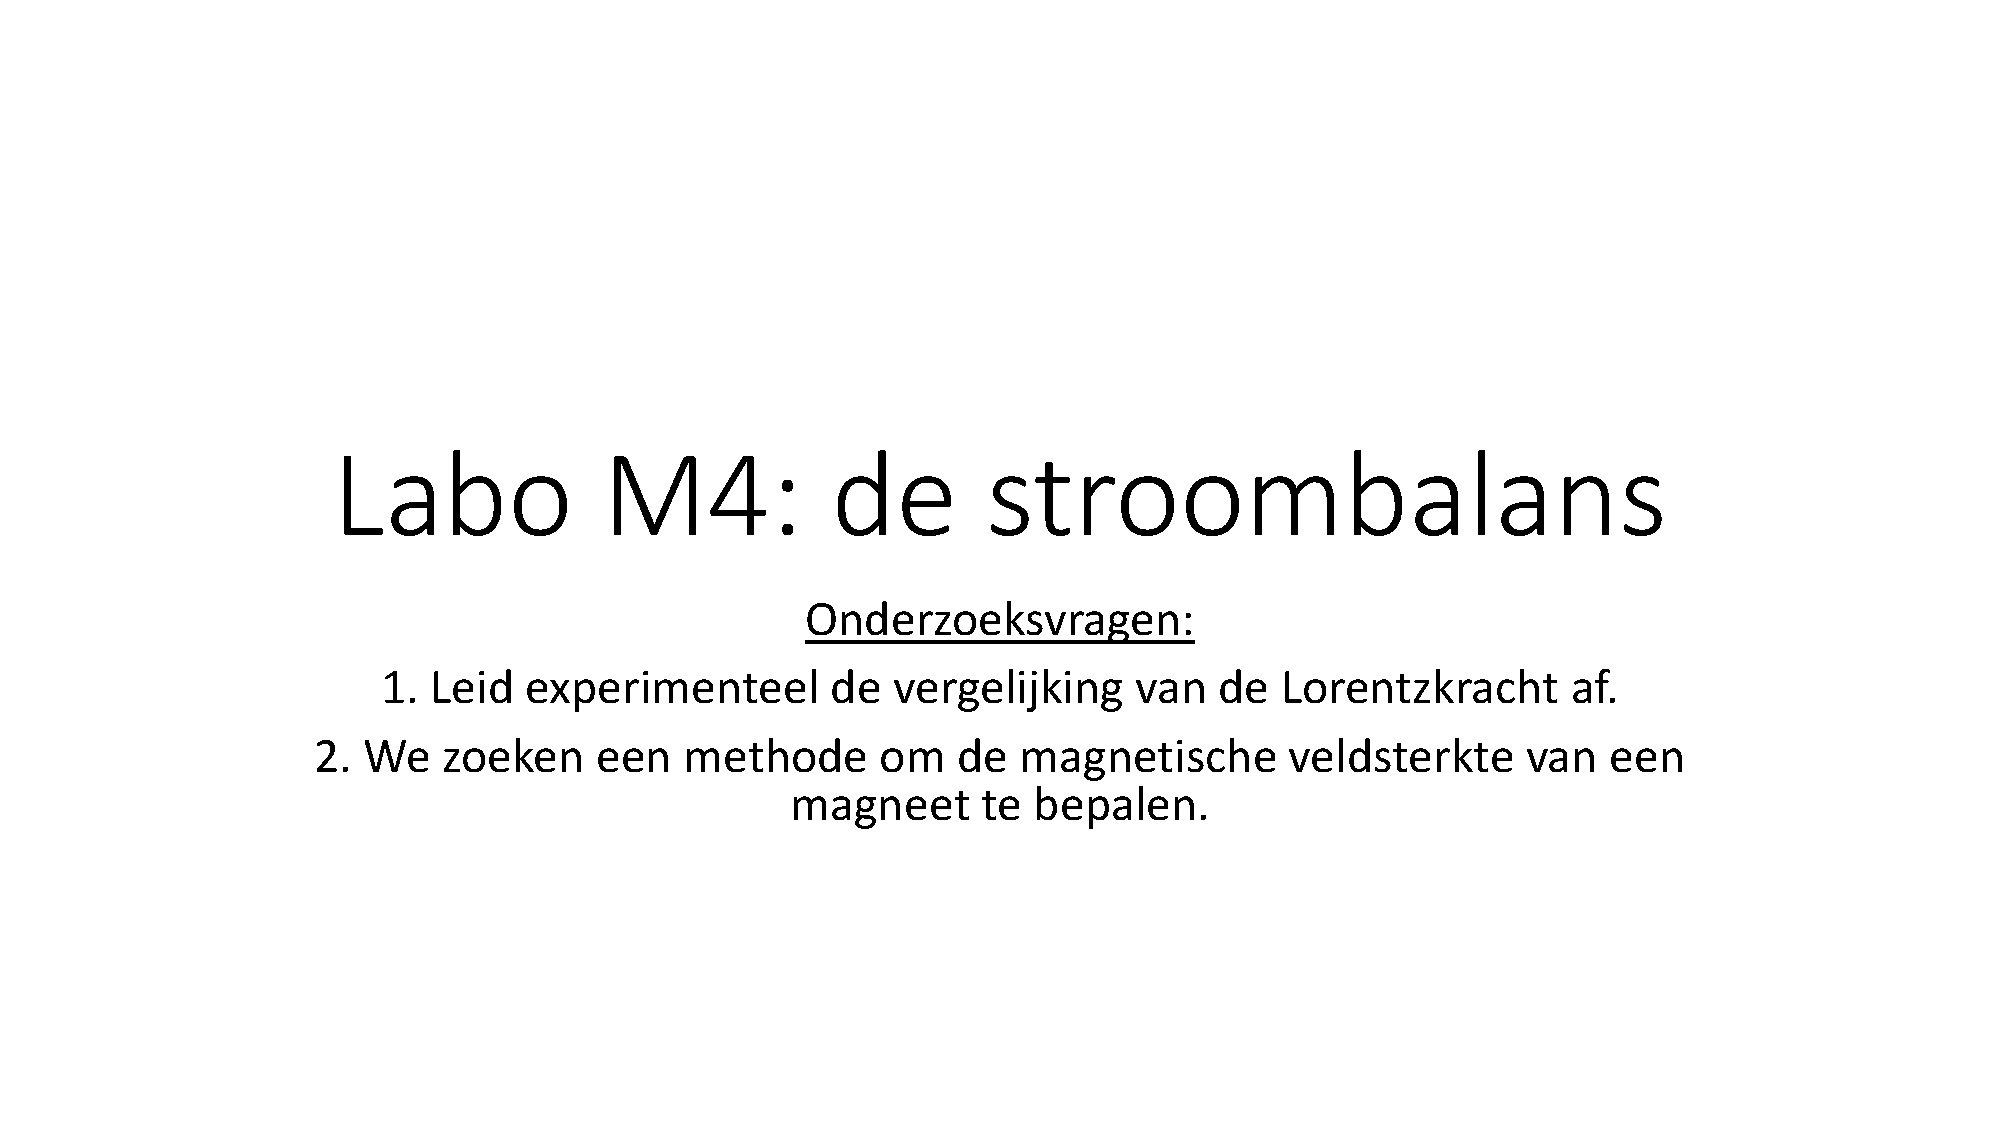
\includepdf[scale = 0.9, pages = -,pagecommand=\subsection*{Bijlage 4.2.5.1: slides bespreking labo},nup=2x3, delta = 0.5cm 1cm]{BesprekingLaboM4.pdf}
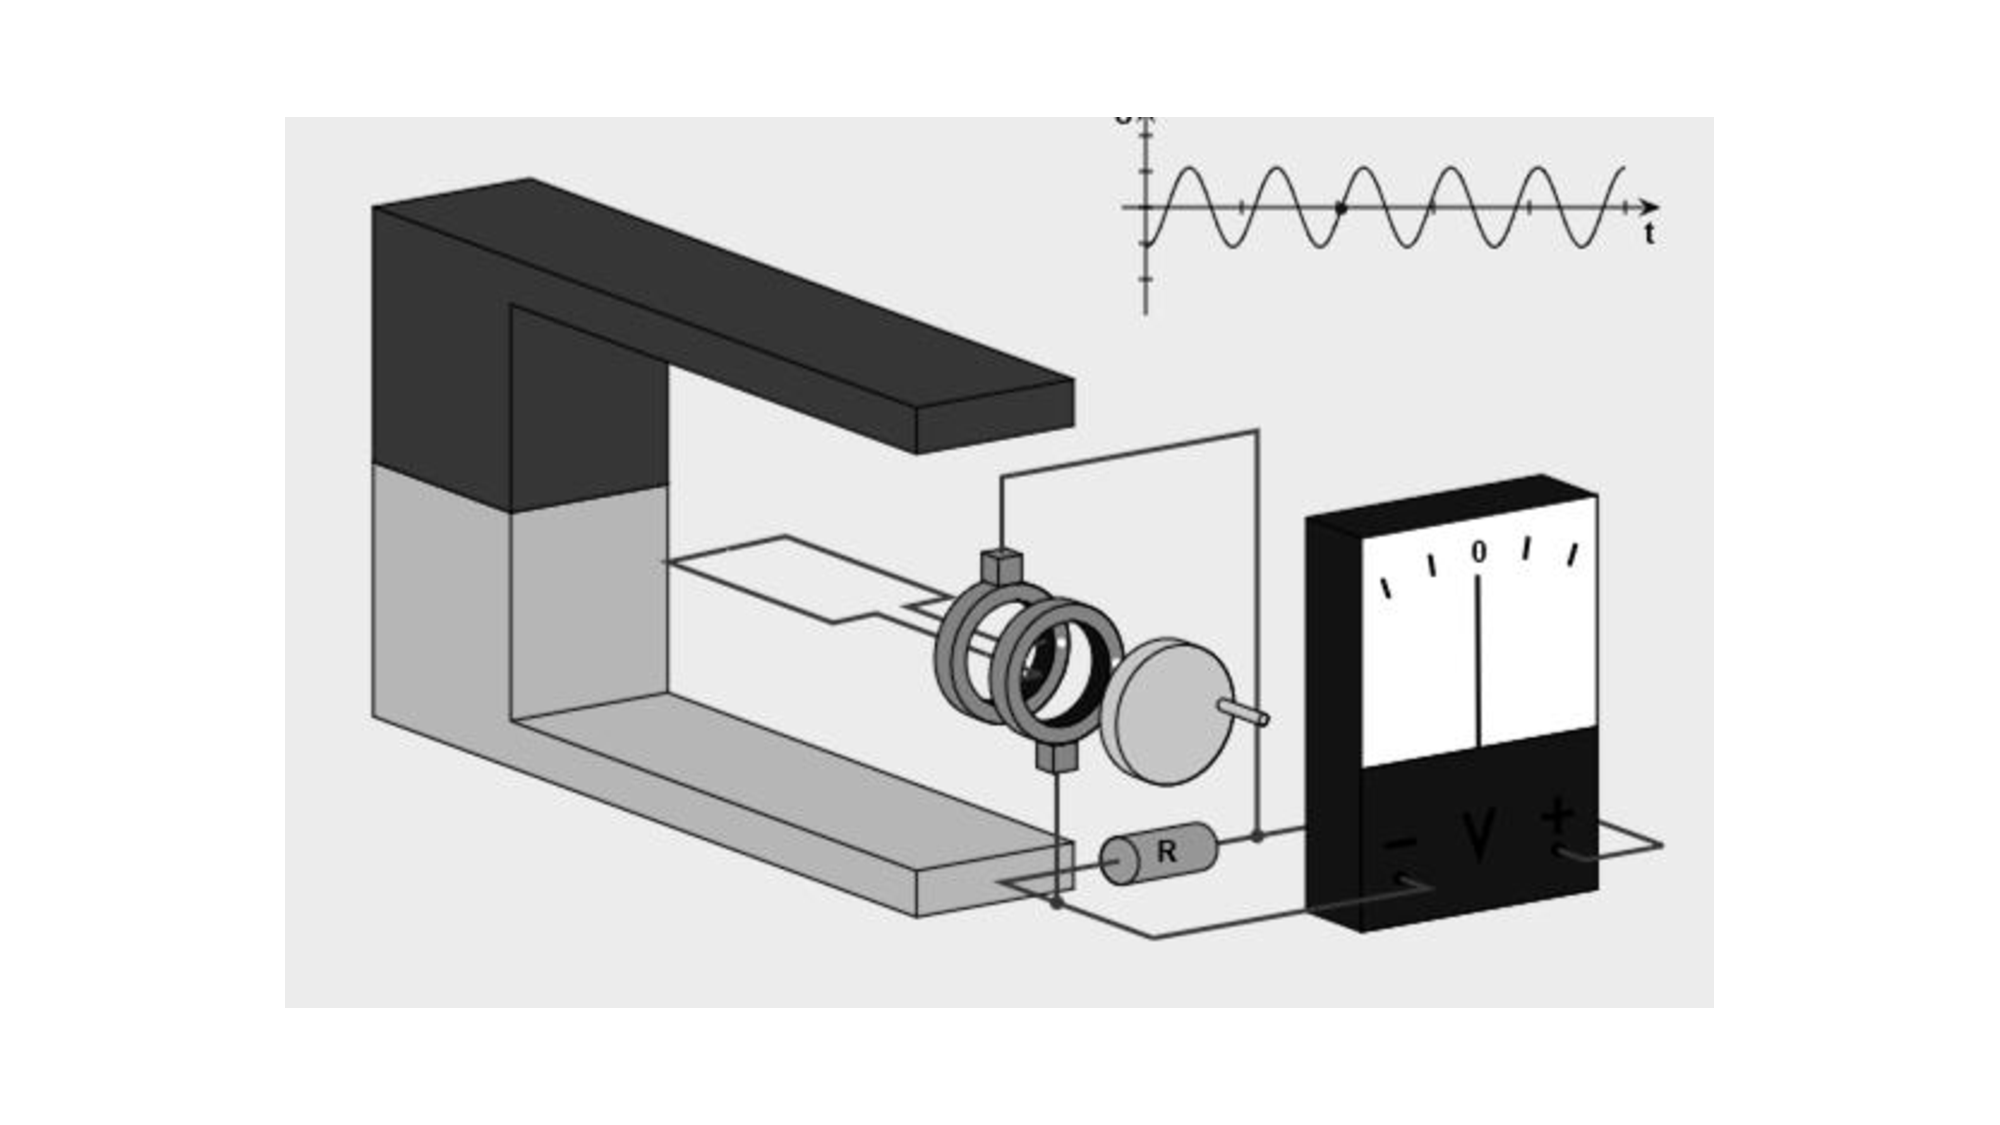
\includepdf[scale = 0.9, pages = -,pagecommand=\subsection*{Bijlage 4.2.5.2: slides bespreking wisselspanningsgenerator},nup=2x3, delta = 0.5cm 1cm]{H6.pdf}

%\subsection*{Bijlage 5.1: slides introductie}

%
%\subsection*{Bijlage 1.2: bordschema theorie}
%\begin{center}
%	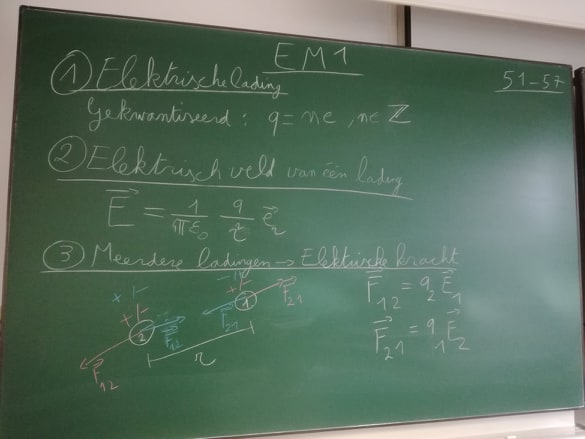
\includegraphics[width=0.9\textwidth]{Bord1a}
%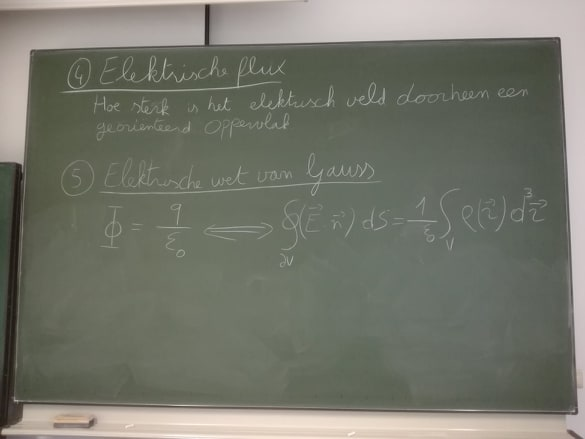
\includegraphics[width=0.9\textwidth]{Bord1b}
%\end{center}
%\newpage
%
%
%\includepdf[scale = 0.8,pages = 17,pagecommand=\subsection*{Bijlage 1.3: opgeloste oefeningen}]{Observaties_OpgelosteOef}
%\includepdf[scale = 0.8,pages =18-20,pagecommand=]{Observaties_OpgelosteOef}
%
%
%
%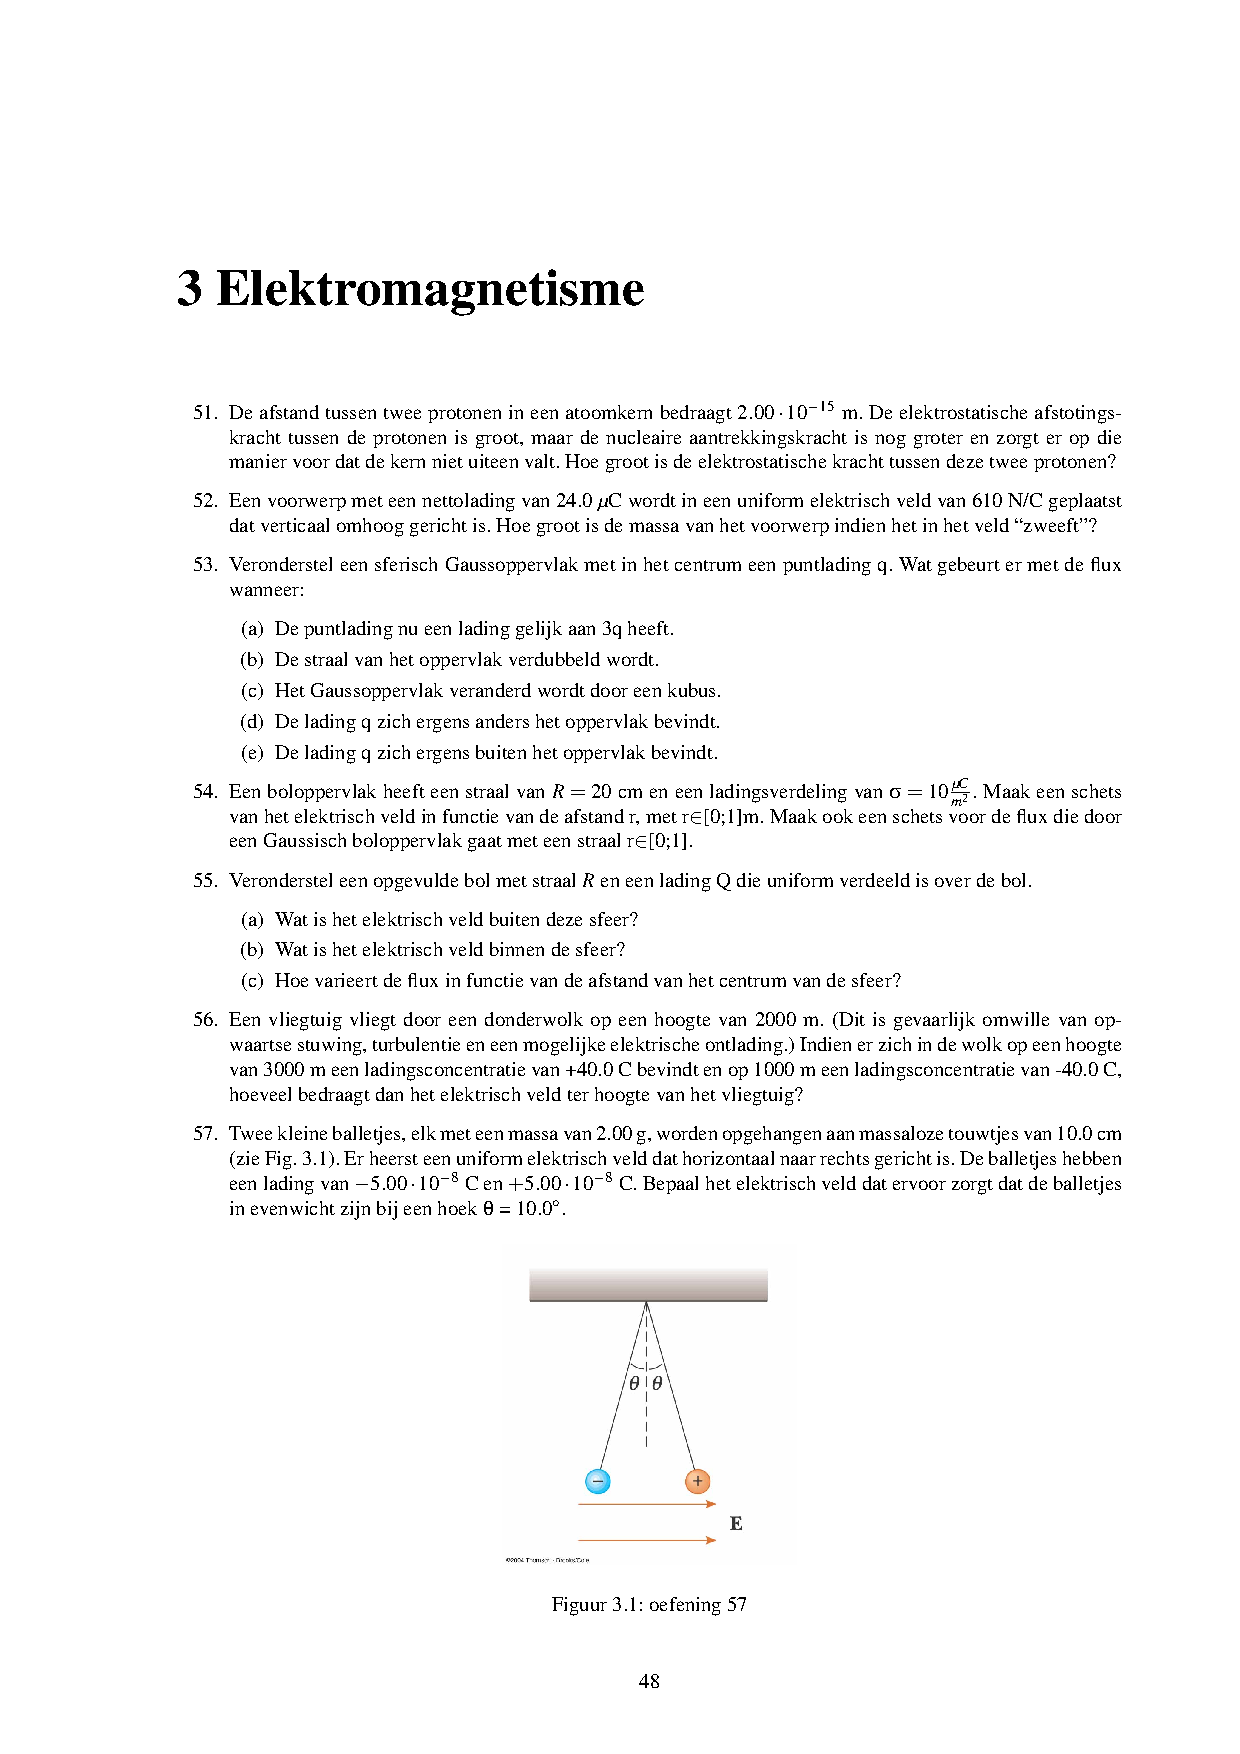
\includepdf[scale = 0.95,pages = 1,pagecommand=\subsection*{Bijlage 1.4: oefeningenbundel elektromagnetisme}]{OefeningenBundel}
%\includepdf[scale = 0.95,pages =2-,pagecommand=]{OefeningenBundel}